\documentclass[a4paper,12pt]{article}
\usepackage[utf8]{inputenc}
\usepackage[spanish]{babel}
\usepackage{amsmath}
\usepackage{siunitx}
\usepackage{geometry}
\usepackage{booktabs}
\usepackage{graphicx}
\usepackage{caption}
\usepackage{pgfplots}
\usepackage{float}

\geometry{margin=2.5cm}
\sisetup{output-decimal-marker = {,}}
\pgfplotsset{compat=1.18}

\begin{document}

% Carátula (completar con los datos del grupo)
\begin{titlepage}
    \centering
    \vspace*{2cm}
    \textbf{\Large Instituto Tecnológico de Buenos Aires} \\
    \vspace{0.5cm}
    \textbf{\large Física III} \\
    \vspace{1cm}
    \textbf{\LARGE Trabajo Práctico N°3 -- Parte 2: Circuitos Rectificadores} \\
    \vspace{1.5cm}
    \begin{tabular}{ll}
        \textbf{Grupo:} & \textit{Completar} \\
        \textbf{Integrantes:} & \textit{Nombre Apellido (Legajo XXXXX)} \\
                              & \textit{Nombre Apellido (Legajo XXXXX)} \\
                              & \textit{Nombre Apellido (Legajo XXXXX)} \\
        \textbf{Fecha de realización:} & \textit{Completar} \\
        \textbf{Fecha de entrega:} & \textit{Completar} \\
    \end{tabular}
    \vspace{2cm}
    \begin{tabular}{|p{12cm}|}
        \hline
        \textbf{Observaciones del docente:} \\
        \vspace{2cm} \\
        \hline
    \end{tabular}
    \vspace{1cm}
    \begin{tabular}{p{6cm}}
        \textbf{Firma del docente:} \\
        \vspace{1cm} \\
        \hrule
    \end{tabular}
\end{titlepage}

\section{Objetivos y Resumen}

Los objetivos específicos de esta segunda parte del trabajo práctico fueron:
\begin{itemize}
    \item Construir y analizar rectificadores de media onda y de onda completa, con y sin capacitor de filtrado, para distintas cargas (resistencia y \emph{cooler}).
    \item Medir la tensión pico a pico de la señal de salida filtrada y de la señal de entrada sin filtrar, para distintos valores de capacitancia.
    \item Evaluar cuantitativamente cómo varía el rizado al cambiar el capacitor y el tipo de rectificación, y comparar los resultados con las expresiones teóricas.
    \item Discernir las diferencias entre tensión pico a pico, tensión promedio y tensión eficaz (RMS) medidas con osciloscopio y multímetro.
\end{itemize}

En las mediciones se observó que, tanto para el rectificador de media onda como para el de onda completa, la inclusión de un capacitor de filtrado reduce fuertemente la tensión de rizado. Para media onda con carga resistiva, el rizado pico a pico disminuyó desde aproximadamente \SI{36,6}{\volt} (sin capacitor) hasta \SI{0,78}{\volt} con el capacitor de mayor valor. Con carga \emph{cooler}, la reducción fue menos marcada debido a la corriente de carga mayor. En el rectificador de onda completa, el rizado con el mismo conjunto de capacitores resultó menor que en media onda, coherente con que la frecuencia del rizado es el doble. Estos resultados son consistentes con la teoría de filtros con capacitor y con el concepto de rizado en fuentes de alimentación.

\begin{figure}[H]
    \centering
    \IfFileExists{foto_montaje_general_rectificadores}{
        \includegraphics[width=0.8\textwidth]{foto_montaje_general_rectificadores}
    }{
        \fbox{Archivo \texttt{foto\_montaje\_general\_rectificadores} no encontrado}
    }
    \caption{Montaje general de los circuitos rectificadores sobre la protoboard. \textit{(Agregar foto correspondiente con este nombre de archivo.)}}
\end{figure}

\section{Introducción Teórica}

\subsection{Rectificación de media onda y de onda completa}

Una fuente de tensión alterna sinusoidal puede modelarse como
\[
v_s(t) = V_{\text{p}} \sin(\omega t),
\]
donde \(V_{\text{p}}\) es la amplitud y \(\omega = 2\pi f\) la frecuencia angular de la red.

En un \textbf{rectificador de media onda} con diodo ideal y carga resistiva, sólo se conduce durante un semiciclo:
\[
v_{\text{o,\,media}}(t) =
\begin{cases}
v_s(t), & \text{si } v_s(t) > 0,\\
0, & \text{si } v_s(t) \le 0.
\end{cases}
\]
La componente continua de la salida (sin filtrado) es
\[
\bar{V}_{\text{o,\,media}} = \frac{V_{\text{p}}}{\pi},
\]
mientras que la tensión eficaz se obtiene integrando el cuadrado de la señal en el periodo.

En un \textbf{rectificador de onda completa} (puente de diodos), ambos semiciclos se “doblan” hacia arriba:
\[
v_{\text{o,\,completa}}(t) = |v_s(t)|,
\]
por lo que la frecuencia de la salida es el doble de la frecuencia de red. En este caso,
\[
\bar{V}_{\text{o,\,completa}} = \frac{2 V_{\text{p}}}{\pi},
\]
y la tensión eficaz también resulta mayor que en el caso de media onda para el mismo valor de \(V_{\text{p}}\).

\begin{figure}[H]
    \centering
    \IfFileExists{esquema_rectificador_media_onda}{
        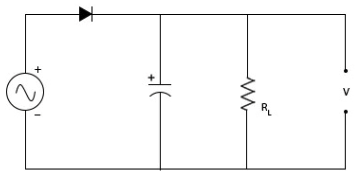
\includegraphics[width=0.8\textwidth]{esquema_rectificador_media_onda}
    }{
        \fbox{Archivo \texttt{esquema\_rectificador\_media\_onda} no encontrado}
    }
    \caption{Esquema del rectificador de media onda con carga resistiva. \textit{(Agregar esquema o foto con este nombre de archivo.)}}
\end{figure}

\begin{figure}[H]
    \centering
    \IfFileExists{esquema_rectificador_onda_completa_puente}{
        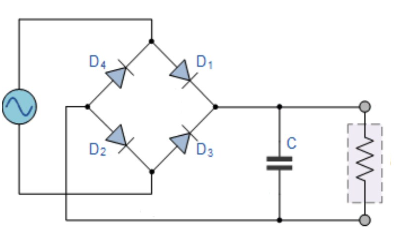
\includegraphics[width=0.8\textwidth]{esquema_rectificador_onda_completa_puente}
    }{
        \fbox{Archivo \texttt{esquema\_rectificador\_onda\_completa\_puente} no encontrado}
    }
    \caption{Esquema del rectificador de onda completa en puente de diodos. \textit{(Agregar esquema o foto con este nombre de archivo.)}}
\end{figure}

\subsection{Capacitor de filtrado y tensión de rizado}

Para obtener una tensión de salida más “continua”, se conecta un capacitor en paralelo con la carga. El capacitor se carga cerca del máximo de la onda rectificada y se descarga a través de la carga durante los intervalos en los que la tensión del rectificador cae por debajo de la tensión almacenada.

Idealizando la descarga del capacitor como aproximadamente lineal entre picos sucesivos, la tensión de rizado pico a pico puede estimarse por
\[
V_{\text{ripple}} \approx \frac{I_{\text{carga}}}{f_{\text{r}}\,C},
\]
donde \(I_{\text{carga}}\) es la corriente media sobre la carga, \(C\) la capacitancia y \(f_{\text{r}}\) la frecuencia de rizado: \(f_{\text{r}} = f\) en media onda y \(f_{\text{r}} = 2f\) en onda completa. A mayor \(C\) o mayor \(f_{\text{r}}\), menor es el rizado esperado.

Es útil expresar la tensión de salida como suma de componente continua y rizado:
\[
v(t) = \bar{V} + v_{\text{rizado}}(t),
\]
donde \(\bar{V}\) es la tensión promedio y \(v_{\text{rizado}}(t)\) tiene valor promedio nulo.

El \textbf{factor de rizado} se define como
\[
r = \frac{V_{\text{rizado,RMS}}}{\bar{V}},
\]
es decir, el cociente entre el valor eficaz del rizado y la componente continua. Aunque en este trabajo no se determinó \(\bar{V}\) numéricamente a partir de las mediciones, la reducción observada en \(V_{\text{ripple}}\) permite discutir cualitativamente el comportamiento de \(r\).

\subsection{Tensión pico, promedio y eficaz}

En señales periódicas no senoidales (como las salidas rectificadas) es importante distinguir entre:
\begin{itemize}
    \item \textbf{Tensión pico (\(V_{\text{p}}\))}: máximo valor instantáneo.
    \item \textbf{Tensión pico a pico (\(V_{\text{pp}}\))}: diferencia entre máximo y mínimo.
    \item \textbf{Tensión promedio (\(\bar{V}\))}: valor medio sobre un periodo.
    \item \textbf{Tensión eficaz (\(V_{\text{RMS}}\))}: valor que produciría la misma potencia en una resistencia que una tensión continua constante.
\end{itemize}

Para una forma de onda genérica \(v(t)\) de periodo \(T\),
\[
V_{\text{RMS}} = \sqrt{\frac{1}{T}\int_0^{T} v^2(t)\, dt}.
\]

Los multímetros suelen mostrar el valor eficaz (o el promedio rectificado equivalente), mientras que el osciloscopio permite acceder directamente a \(V_{\text{p}}\) y \(V_{\text{pp}}\), y en muchos casos también a \(V_{\text{RMS}}\) calculado numéricamente.

\section{Instrumentos, Elementos y Procedimiento Experimental}

\subsection{Instrumentos y elementos}

\begin{itemize}
    \item Fuente de alterna (\emph{transformador} o fuente de laboratorio) de aproximadamente \SI{12}{\volt} RMS a \SI{50}{\hertz}.
    \item Diodos para rectificación (por ejemplo, 1N4007) para el rectificador de media onda y el puente de onda completa.
    \item Resistencias de carga (por ejemplo, \(R \approx \SI{100}{\ohm}\)). \textit{(Completar con el valor exacto utilizado.)}
    \item Carga \emph{cooler} (motor/ventilador de PC).
    \item Capacitores de filtrado \(C_1\), \(C_2\) y \(C_3\). \textit{(Completar con los valores nominales, por ejemplo en \si{\micro\farad}.)}
    \item Osciloscopio digital para medir formas de onda y amplitudes pico a pico.
    \item Multímetro para verificar valores medios o eficaces de tensión.
    \item Protoboard, cables y puntas de prueba.
\end{itemize}

\begin{figure}[H]
    \centering
    \IfFileExists{foto_montaje_media_onda_resistencia}{
        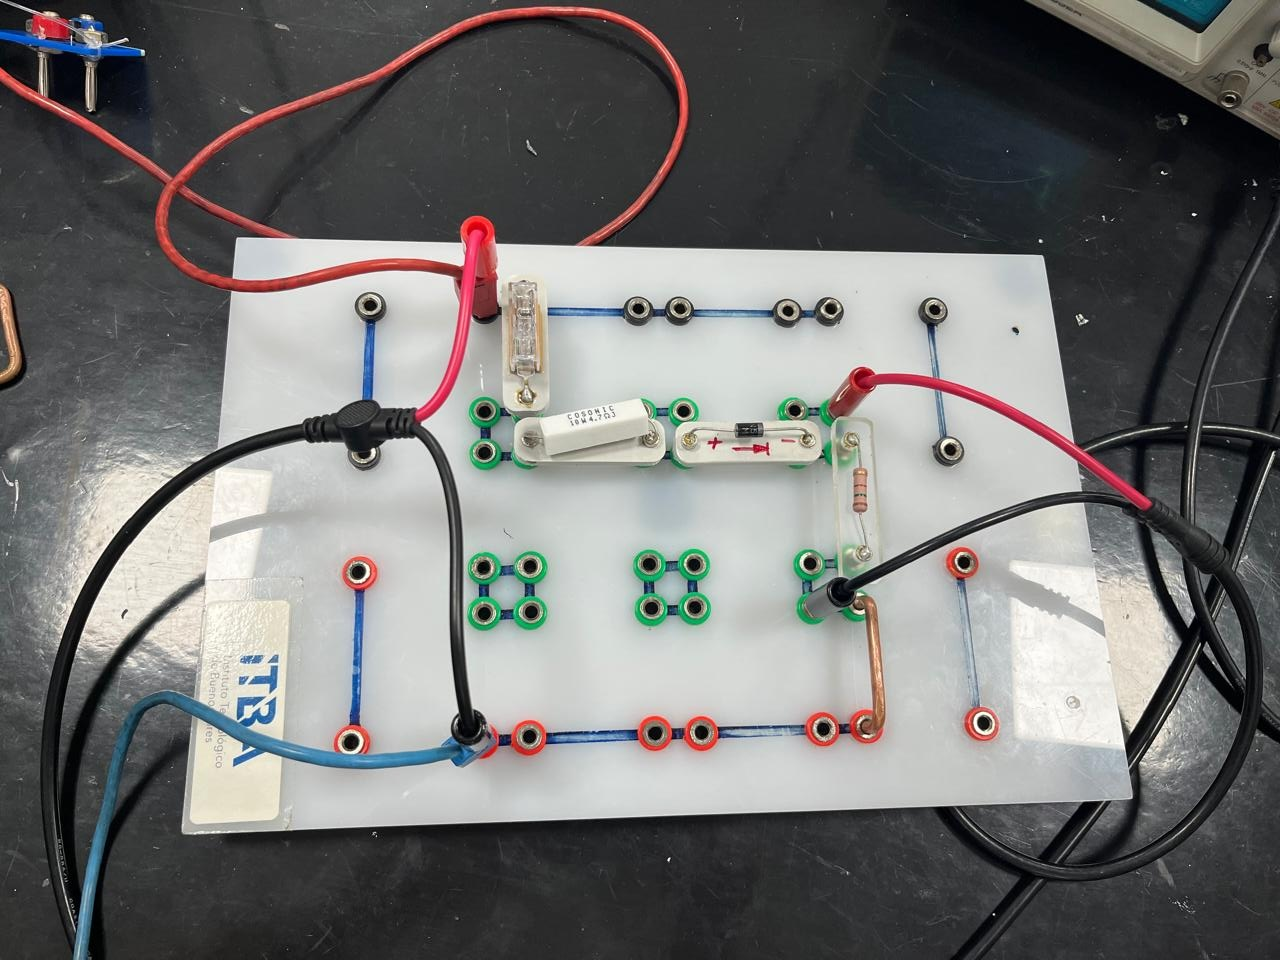
\includegraphics[width=0.8\textwidth]{foto_montaje_media_onda_resistencia}
    }{
        \fbox{Archivo \texttt{foto\_montaje\_media\_onda\_resistencia} no encontrado}
    }
    \caption{Montaje del rectificador de media onda con carga resistiva. \textit{(Agregar foto correspondiente con este nombre de archivo.)}}
\end{figure}

\begin{figure}[H]
    \centering
    \IfFileExists{foto_montaje_media_onda_cooler}{
        \includegraphics[width=0.8\textwidth]{foto_montaje_media_onda_cooler}
    }{
        \fbox{Archivo \texttt{foto\_montaje\_media\_onda\_cooler} no encontrado}
    }
    \caption{Montaje del rectificador de media onda con carga \emph{cooler}. \textit{(Agregar foto correspondiente con este nombre de archivo.)}}
\end{figure}

\begin{figure}[H]
    \centering
    \IfFileExists{foto_montaje_onda_completa_puente}{
        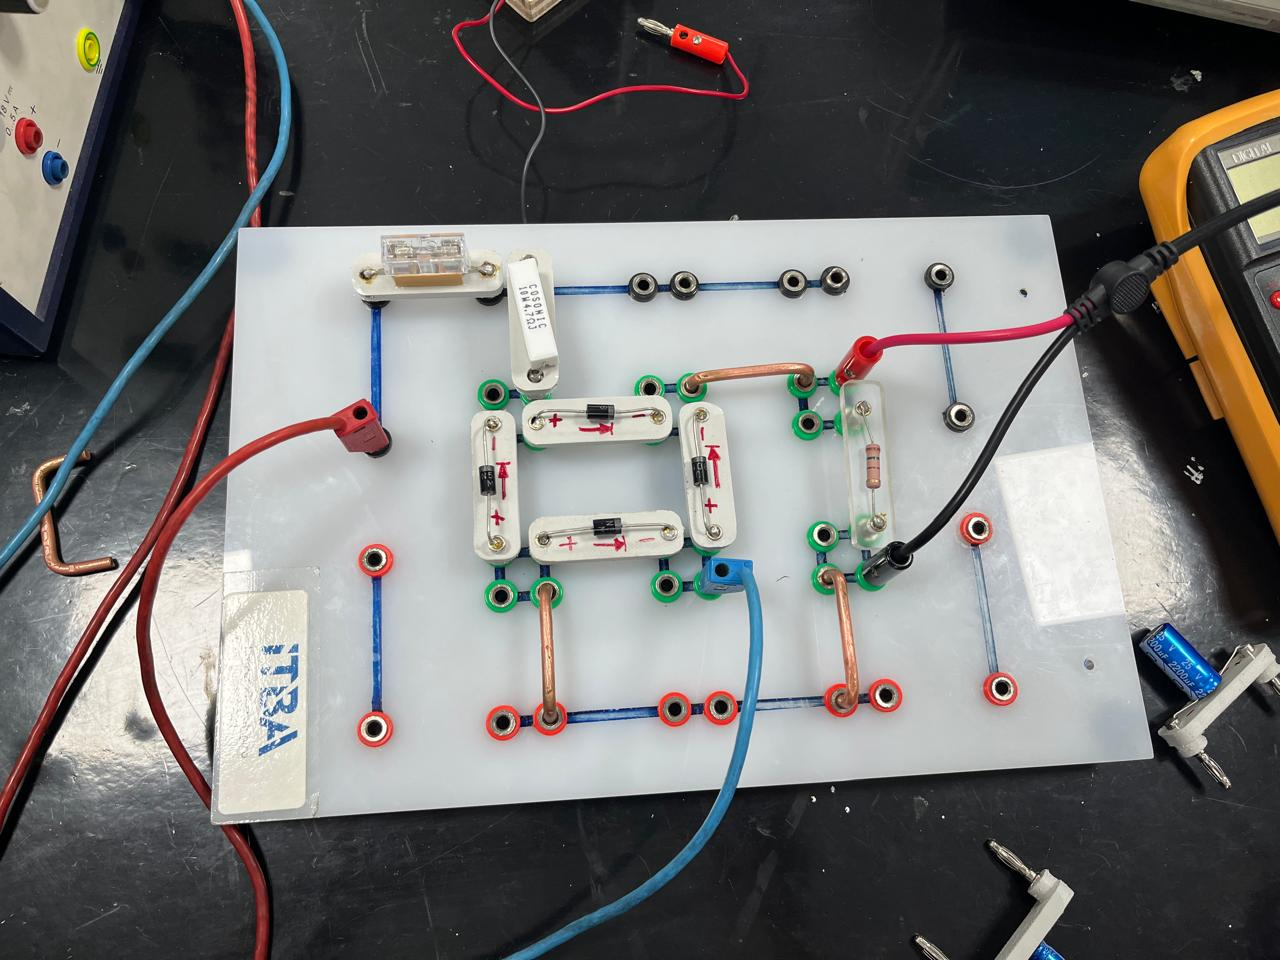
\includegraphics[width=0.8\textwidth]{foto_montaje_onda_completa_puente}
    }{
        \fbox{Archivo \texttt{foto\_montaje\_onda\_completa\_puente} no encontrado}
    }
    \caption{Montaje del rectificador de onda completa en puente de diodos. \textit{(Agregar foto correspondiente con este nombre de archivo.)}}
\end{figure}

\subsection{Procedimiento experimental}

\subsubsection*{Rectificador de media onda con carga resistiva}
\begin{enumerate}
    \item Se armó el rectificador de media onda con un diodo y la resistencia de carga \(R\).
    \item Sin capacitor de filtrado, se observó la forma de onda de salida en el osciloscopio y se midió la tensión pico a pico de la señal de entrada sin filtrar.
    \item Se conectó el capacitor \(C_1\) en paralelo con la carga y se midió \(V_{\text{pp}}\) de la onda filtrada.
    \item Se repitió el procedimiento para los capacitores \(C_2\) y \(C_3\).
\end{enumerate}

\subsubsection*{Rectificador de media onda con carga \emph{cooler}}
\begin{enumerate}
    \item Se reemplazó la resistencia de carga por el \emph{cooler}.
    \item Sin capacitor, se midió la tensión pico a pico de la señal de entrada sin filtrar.
    \item Se conectaron sucesivamente los capacitores \(C_1\), \(C_2\) y \(C_3\) en paralelo con el \emph{cooler}, midiendo en cada caso el \(V_{\text{pp}}\) de la señal filtrada.
    \item Se comparó cualitativamente la velocidad de giro del \emph{cooler} entre las distintas configuraciones.
\end{enumerate}

\subsubsection*{Rectificador de onda completa con filtrado capacitivo}
\begin{enumerate}
    \item Se armó un rectificador de onda completa en puente de diodos, con la misma fuente de alterna y la misma resistencia de carga utilizada en la sección de media onda.
    \item Sin capacitor, se midió el \(V_{\text{pp}}\) de la señal rectificada.
    \item Se conectaron los capacitores \(C_1\), \(C_2\) y \(C_3\) en paralelo con la carga, registrando el \(V_{\text{pp}}\) de la señal filtrada en cada caso.
    \item Se comparó el rizado observado en el osciloscopio para media onda y onda completa.
\end{enumerate}

\section{Datos Obtenidos y Análisis}

En esta sección se presentan las mediciones de tensión pico a pico tanto de la señal filtrada como de la señal de entrada sin filtrar, utilizando los datos del archivo \texttt{MEDICIONES F3  - TP3P2Data.csv}.

\subsection{Rectificador de media onda con carga resistiva}

Para esta configuración se midió la tensión pico a pico de la señal de entrada sin filtrar y de la señal filtrada para distintos capacitores.

\begin{table}[H]
    \centering
    \begin{tabular}{lcc}
        \toprule
        Configuración & $V_{\text{pp, filtrada}}$ (\si{\volt}) & $V_{\text{pp, entrada}}$ (\si{\volt}) \\
        \midrule
        Sin capacitor & --   & 36,6 \\
        Con $C_1$     & 12,1 & --   \\
        Con $C_2$     & 6,7  & --   \\
        Con $C_3$     & 0,78 & --   \\
        \bottomrule
    \end{tabular}
    \caption{Tensiones pico a pico medidas en el rectificador de media onda con carga resistiva.}
\end{table}

Tomando como referencia la tensión pico a pico de entrada sin filtrar (\(\approx \SI{36,6}{\volt}\)), se puede estimar una reducción relativa del rizado para cada capacitor:
\begin{itemize}
    \item $C_1$: $V_{\text{ripple}} \approx \SI{12,1}{\volt}$, es decir, alrededor del 33 \% del valor de referencia.
    \item $C_2$: $V_{\text{ripple}} \approx \SI{6,7}{\volt}$, aproximadamente un 18 \%.
    \item $C_3$: $V_{\text{ripple}} \approx \SI{0,78}{\volt}$, cerca de un 2 \%.
\end{itemize}

La fuerte reducción del rizado al aumentar la capacitancia es coherente con la relación inversa \(V_{\text{ripple}} \propto 1/C\).

\begin{figure}[H]
    \centering
    \begin{tikzpicture}
        \begin{axis}[
            ybar,
            ymin=0,
            ylabel={$V_{\text{pp}}$ (\si{\volt})},
            symbolic x coords={Sin C,C1,C2,C3},
            xtick=data,
            width=0.8\textwidth,
            height=0.4\textwidth,
            legend style={at={(0.5,-0.2)},anchor=north,legend columns=-1},
            ylabel style={font=\small},
            xticklabel style={font=\small, rotate=0},
        ]
            \addplot coordinates {(Sin C,36.6) (C1,12.1) (C2,6.7) (C3,0.78)};
        \end{axis}
    \end{tikzpicture}
    \caption{Evolución de la tensión pico a pico en media onda con carga resistiva al variar el capacitor de filtrado.}
\end{figure}

\begin{figure}[H]
    \centering
    \IfFileExists{oscilograma_media_onda_resistencia_C3}{
        \includegraphics[width=0.8\textwidth]{oscilograma_media_onda_resistencia_C3}
    }{
        \fbox{Archivo \texttt{oscilograma\_media\_onda\_resistencia\_C3} no encontrado}
    }
    \caption{Oscilograma de la salida del rectificador de media onda con carga resistiva y capacitor $C_3$ (máxima filtración). \textit{(Agregar captura de pantalla con este nombre de archivo.)}}
\end{figure}

\subsection{Rectificador de media onda con carga \emph{cooler}}

En esta configuración, la carga es un \emph{cooler} que demanda una corriente mayor y presenta componentes inductivas. Las mediciones fueron:

\begin{table}[H]
    \centering
    \begin{tabular}{lcc}
        \toprule
        Configuración & $V_{\text{pp, filtrada}}$ (\si{\volt}) & $V_{\text{pp, entrada}}$ (\si{\volt}) \\
        \midrule
        Sin capacitor & --   & 36,2 \\
        Con $C_1$     & 16,1 & --   \\
        Con $C_2$     & 13,0 & --   \\
        Con $C_3$     & 8,4  & --   \\
        \bottomrule
    \end{tabular}
    \caption{Tensiones pico a pico medidas en el rectificador de media onda con carga \emph{cooler}.}
\end{table}

Comparando con la referencia sin capacitor (\(\approx \SI{36,2}{\volt}\)):
\begin{itemize}
    \item \(C_1\): rizado \(\approx 16,1/36,2 \approx 0,44\).
    \item \(C_2\): rizado \(\approx 13,0/36,2 \approx 0,36\).
    \item \(C_3\): rizado \(\approx 8,4/36,2 \approx 0,23\).
\end{itemize}

Si bien el rizado disminuye con el aumento de la capacitancia, el efecto es menos drástico que con la carga puramente resistiva. Esto se debe principalmente a la mayor corriente de carga y a la naturaleza no puramente resistiva del \emph{cooler}, que incrementan la descarga del capacitor entre picos.

En la práctica, se observó que la velocidad del \emph{cooler} aumenta al utilizar capacitores de mayor valor, reflejando una tensión más constante y un menor rizado.

\begin{figure}[H]
    \centering
    \IfFileExists{oscilograma_media_onda_cooler_sin_C}{
        \includegraphics[width=0.8\textwidth]{oscilograma_media_onda_cooler_sin_C}
    }{
        \fbox{Archivo \texttt{oscilograma\_media\_onda\_cooler\_sin\_C} no encontrado}
    }
    \caption{Oscilograma de la salida del rectificador de media onda alimentando el \emph{cooler}, sin capacitor de filtrado. \textit{(Agregar captura de pantalla con este nombre de archivo.)}}
\end{figure}

\subsection{Rectificador de onda completa}

Para el rectificador de onda completa en puente, se obtuvieron los siguientes valores de tensión pico a pico en la salida:

\begin{table}[H]
    \centering
    \begin{tabular}{lcc}
        \toprule
        Configuración & $V_{\text{pp, filtrada}}$ (\si{\volt}) & $V_{\text{pp, entrada}}$ (\si{\volt}) \\
        \midrule
        Sin capacitor & 16,1 & --   \\
        Con $C_1$     & 6,56 & --   \\
        Con $C_2$     & 3,04 & --   \\
        Con $C_3$     & 0,57 & --   \\
        \bottomrule
    \end{tabular}
    \caption{Tensiones pico a pico medidas en el rectificador de onda completa.}
\end{table}

Tomando como referencia el caso sin capacitor (\(\approx \SI{16,1}{\volt}\)):
\begin{itemize}
    \item \(C_1\): rizado \(\approx 6,56/16,1 \approx 0,41\).
    \item \(C_2\): rizado \(\approx 3,04/16,1 \approx 0,19\).
    \item \(C_3\): rizado \(\approx 0,57/16,1 \approx 0,035\).
\end{itemize}

La reducción del rizado es notablemente eficiente en onda completa, especialmente para el capacitor de mayor valor, donde el rizado es de apenas algunos puntos porcentuales. Esto concuerda con la expresión teórica, dado que en onda completa la frecuencia de rizado es \(2f\), lo que reduce en un factor 2 el rizado esperado frente a media onda para el mismo \(C\) e \(I_{\text{carga}}\).

\begin{figure}[H]
    \centering
    \begin{tikzpicture}
        \begin{axis}[
            ybar,
            ymin=0,
            ylabel={$V_{\text{pp}}$ (\si{\volt})},
            symbolic x coords={Sin C,C1,C2,C3},
            xtick=data,
            width=0.8\textwidth,
            height=0.4\textwidth,
            legend style={at={(0.5,-0.2)},anchor=north,legend columns=-1},
            ylabel style={font=\small},
            xticklabel style={font=\small, rotate=0},
        ]
            \addplot coordinates {(Sin C,16.1) (C1,6.56) (C2,3.04) (C3,0.57)};
        \end{axis}
    \end{tikzpicture}
    \caption{Tensión pico a pico en el rectificador de onda completa al variar el capacitor de filtrado.}
\end{figure}

\section{Discusión de Resultados}

\subsection{Efecto del capacitor de filtrado}

En todas las configuraciones se verifica que el aumento de la capacitancia reduce el rizado, tal como predice
\[
V_{\text{ripple}} \approx \frac{I_{\text{carga}}}{f_{\text{r}}\,C}.
\]
Aunque no se calcularon \(I_{\text{carga}}\) ni los valores exactos de \(C_1\), \(C_2\) y \(C_3\) en este informe, la variación de \(V_{\text{pp}}\) medida es compatible con una disminución aproximadamente proporcional a \(1/C\), especialmente entre \(C_1\) y \(C_3\).

\subsection{Comparación media onda vs. onda completa}

Para un mismo orden de magnitud de los capacitores, el rectificador de onda completa presenta una tensión de rizado menor que el de media onda. Esto se debe a que el tiempo de descarga del capacitor entre picos de tensión es menor (la onda rectificada de onda completa tiene frecuencia \(2f\)), de modo que la caída de tensión entre picos es reducida.

Además, el valor medio de la tensión de salida en onda completa es mayor, lo que mejora la eficiencia de la conversión AC--DC.

\subsection{Carga resistiva vs. carga \emph{cooler}}

Comparando las tablas de media onda, se observa que, para un mismo capacitor, el rizado con carga \emph{cooler} es mayor que con carga resistiva. Esto es coherente con una corriente media más alta a través del capacitor: mayor corriente implica una descarga más rápida entre picos, y por lo tanto un \(V_{\text{ripple}}\) mayor.

En términos cualitativos, la velocidad de giro del \emph{cooler} aumenta al incrementar la capacitancia, ya que la tensión de alimentación se vuelve más cercana a una continua pura.

\subsection{Mediciones con osciloscopio y multímetro}

En el osciloscopio se midieron principalmente tensiones pico a pico, mientras que el multímetro reporta valores eficaces o promedios (según el modo de medición). En señales muy rizadas, el valor mostrado por el multímetro puede diferir significativamente de la componente continua ideal, ya que integra tanto la componente continua como el rizado.

En cambio, al aumentar la capacitancia y reducir el rizado, el valor medido por el multímetro se aproxima más a la tensión continua esperada a la salida del rectificador filtrado.

\section{Aplicaciones Prácticas}

Los rectificadores con filtrado capacitivo son la base de las fuentes de alimentación lineales utilizadas en numerosos dispositivos electrónicos (cargadores, adaptadores, fuentes de laboratorio sencillas, etc.). En ellas, el diseño del capacitor de filtrado debe balancear el rizado tolerable, el tamaño del capacitor y el costo.

Los resultados obtenidos muestran en forma directa cómo el aumento de la capacitancia y el uso de rectificación de onda completa permiten reducir el rizado a valores compatibles con el funcionamiento de cargas sensibles, como circuitos electrónicos o motores de corriente continua de baja potencia.

\section{Conclusiones}

En esta segunda parte del trabajo práctico se estudiaron experimentalmente rectificadores de media onda y de onda completa, con distintas cargas y capacitores de filtrado. Las mediciones de tensión pico a pico mostraron que:
\begin{itemize}
    \item El rizado disminuye al aumentar la capacitancia del filtro.
    \item El rectificador de onda completa presenta un rizado menor que el de media onda para la misma carga y el mismo capacitor, en concordancia con la teoría.
    \item La carga \emph{cooler} introduce un rizado mayor que la carga puramente resistiva, debido a la mayor corriente de carga.
\end{itemize}

En conjunto, el experimento permitió validar cualitativamente las expresiones teóricas para el rizado y resaltar la importancia del diseño del filtro capacitivo en fuentes de alimentación basadas en rectificadores.

\end{document}

